\documentclass[12pt]{article}

\input quiz-setup
\usepackage{mdframed}%can make highlighted boxes of text
%Use case: https://tex.stackexchange.com/questions/46828/how-to-highlight-important-parts-with-a-gray-background
\newcommand{\version}{} 
\newcommand{\xzero}{}
\newcommand{\xone}{}
\newcommand{\xtwo}{}
\newcommand{\xthree}{}
\newcommand{\xfour}{}
\newcommand{\xfive}{}

\newcommand{\ExamName}{Quiz \#4\version}
% \newcommand{\CourseName}{Math 34A}
% \renewcommand{\Quarter}{Spring 2017}

%\begin{highlight}...\end{highlight} Puts a gray box around something you want to stand out.
\newenvironment{highlight}{\begin{mdframed}[backgroundcolor=gray!20]}{\end{mdframed}}



\begin{document}
%%
%% Version A:
\renewcommand{\version}{}
\renewcommand{\xzero}{0.0}
\renewcommand{\xone}{1.3}
\renewcommand{\xtwo}{2.9}
\renewcommand{\xthree}{4.1}
\renewcommand{\xfour}{5.3}
\renewcommand{\xfive}{6.5}
% 
\begin{minipage}{0.25\linewidth}
  \CourseName\ \Quarter \\
  \ExamName \\[1em]
  \textbf{No calculators}\\[2em]
\end{minipage}
\hfill
\begin{minipage}[t]{0.4\linewidth}
  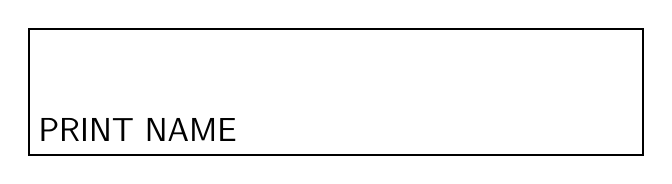
\begin{tikzpicture}[x=26mm,y=16mm]
    \draw[thick,black] (0,0) rectangle (3,1);
    \node[\faintcolor,right] at (0,0.2) {\large\textsf{PRINT NAME}};
  \end{tikzpicture}
\end{minipage}
\hfill
\begin{minipage}{0.25\linewidth}
  \vspace*{-3.25em}
  \ \hfill
  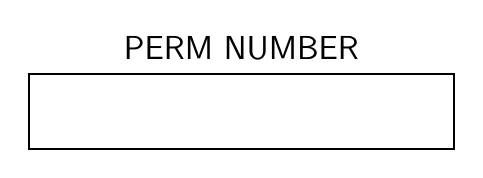
\begin{tikzpicture}[x=36mm,y=16mm]
    \node[\faintcolor] at (0.75,0.8) {\large\textsf{PERM NUMBER}};
    \draw[thick,black] (0,0) rectangle (1.5,0.6);
  \end{tikzpicture}
\end{minipage}
% \medskip
\vspace*{-0.25in}

Put your answer in the 
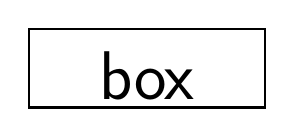
\begin{tikzpicture}[x=10mm,y=10mm,baseline=3mm] 
  \draw[thick,black] (0,0) rectangle (3,1);
  \node[\faintcolor] at (1.5,0.4) {\Huge\textsf{box}};
\end{tikzpicture}
provided.
\hfill
\begin{minipage}{0.5\linewidth}
\begin{center}

  \textbf{TA:}\ 
  \parbox[t]{0.7in}{%
    \checkbox\ \TAOne \\
    \checkbox\ \TATwo 
  }
  %\parbox[t]{0.7in}{%
  %  \checkbox\ \TAThree\\
  %  \ \ \ 
  %}
  % \ 
  % \parbox[t]{4in}{%
  % \textbf{Section Time:}
  \hfill%\hspace*{0.25in}
  % \ 
  % \parbox[t]{4in}{%
  % \textbf{Section Time:}
  \textbf{Time:}
  \parbox[t]{0.55in}{%
    \checkbox\ 4:30 \\
    \checkbox\ 5:30
  }
  \quad
  \parbox[t]{0.55in}{%
    \checkbox\ 6:30 \\
    \checkbox\ 7:30 
  }
  % }
%  \textbf{TA:}\ 
%  \parbox[t]{0.95in}{%
%    \checkbox\ \TAOne
%  }
%  \parbox[t]{0.95in}{%
%    \checkbox\ \TATwo\\
%  }
%%  \parbox[t]{0.95in}{%
%%    \checkbox\ \TAThree
%%  }
%  \hspace*{0.5in} 
%  \parbox[t]{3in}{%
%    \textbf{Section Time:}
%    \parbox[t]{0.75in}{%
%      \checkbox\ 4:30 \\
%      \checkbox\ 5:30
%    }
%    \parbox[t]{0.75in}{%
%      \checkbox\ 6:30 \\
%      \checkbox\ 7:30
%    }
%  }
\end{center}

\end{minipage}
\noindent\hspace*{-2em}\rule{\textwidth+4em}{1pt}%

\mbox{}

{\large \textbf{Variation of Parameters}}

\bigskip
Following is the formula for the variation of parameters method, which we will explore in today's quiz. I have suppressed the notation a bit, to make it easier to read and remember. 

\begin{highlight}
For an ODE of the form 
$$y''+p(t)y'+q(t)y=g(t)$$
with homogeneous solution %\footnote{Here ``homogeneous solution" means the general solution of the corresponding homogeneous equation $y''+p(t)y'+q(t)y=0$.}
$$y_h=C_1y_1+C_2y_2,$$ 
you can find a particular solution by
$$y_p = -y_1\int\frac{y_2g}{W} + y_2\int\frac{y_1g}{W}$$
where $W$ is the Wronskian $W[y_1,y_2]$. 

\bigskip The general solution can be found by adding these together:
$$y_g=y_h+y_p.$$
\end{highlight}

Let's try a step-by-step example.

\begin{enumerate}
  \setcounter{problemnumber}{0}
	\Problem Find a general solution to the following differential equation.
	$$y''+9y=3\tan(3t)$$
	\begin{enumerate}
		\item First we find $y_h$. To do this, find the general solution to 
		$y''+9y=0$. 
		\begin{flushright}
		$y_h=$ \answerbox{8}
		\end{flushright}
		\vfill
		
		\pagebreak
		\item Next we're going to use the formula $y_p = -y_1\int\frac{y_2g}{W} + y_2\int\frac{y_1g}{W}$, so let's compute the Wronskian $W[y_1, y_2]$	and write down everything we'll need to plug in:
		
		$\hfill y_1= \answerbox{3} 
		\hfill y_2= \answerbox{3} 
		\hfill g= \answerbox{3} 
		\hfill W= \answerbox{3} 
		\hfill $
		\vfill
		
		\item Now let's use the formula 
		$$ y_p = -y_1\int\frac{y_2g}{W} + y_2\int\frac{y_1g}{W}.$$
		By the way, there's no need to worry about $+C$ for the integrals in this formula.\footnote{This is because when we want the most general solution, adding $y_h$ does for us what $+C$ does for an indefinite integral.}
		
		To make it a little easier to break up into steps, let's call $\displaystyle u_1=-\int\frac{y_2g}{W}$ and $\displaystyle u_2=\int\frac{y_1g}{W}$ so that 
		$$y_p = y_1u_1 + y_2u_2.$$
		
		\item[] Find $\displaystyle u_1=-\int\frac{y_2g}{W}$. %u_1
		
		{\small [Hint: put everything in terms of $\cos$ and use the fact that $\int\frac{1}{\cos(x)}=\ln|\sec(x)+\tan(x)|$]}
		\begin{flushright}
		$u_1=$ \answerbox{8}
		\end{flushright}
		\vfill
		\vfill		
		
		\item Find $\displaystyle u_2=\int\frac{y_1g}{W}$. %u_2
		\begin{flushright}
		$u_2=$ \answerbox{8}
		\end{flushright}
		\vfill
		
		
		\pagebreak		
		\item Now we write $y_p=y_1u_1+y_2u_2$ and simplify.
		\begin{flushright}
		$y_p=$ \answerbox{12}
		\end{flushright}
		\vspace*{72pt}

		\item To find the general solution, we just write $y_g=y_h+y_p$.
		\begin{flushright}
		$y_g=$ \answerbox{18}
		\end{flushright}		
	\end{enumerate}
	\vspace*{36pt}
	
	\Problem Now try one on your own: 
	$$y''-2y'+y=\frac{e^t}{t^2+1}$$	
	[Hint: start by rewriting the formula from memory as much as possible, so you can work on memorizing it.]
	\begin{flushright}
	$y_g=$ \answerbox{18}
	\end{flushright}		
	\vfill
	
	\pagebreak
	\text{[This page left blank for use as scratch paper]}
	\vfill
    

	
%	\vfill
\end{enumerate}




\end{document}
